\chapter{Project Management}

\section{Overview}

The overall objective of project management is to implement a process to achieve successful completion of the project in terms of \textbf{cost}, \textbf{schedule} and \textbf{technical performance}. Project management is performed following a structured approach throughout all the stages of its life cycle and at all the levels of the \textbf{customer-supplier chain}.

The notation of customer-supplier model\index{Customer-supplier model} is used throughout this book to denote the concept that  the production of a space system involves parties that supply and parties that consume goods and/or services. In its simplest form, a project can comprise one customer with one or more supplier; however, most space projects comprise a number of hierarchical levels, where:

\begin{itemize}
\item the actor at the top level of the hierarchy is the top level customer (i.e. the stakeholder),
\item the actors at intermediate levels of the hierarchy are both supplier and
customer,
\item the actors at the lowest level of the hierarchy are suppliers only.
\end{itemize}

Project management integrates all management, engineering and product assurance functions required to execute the project.

\subsection{Project Initiation} 

Initially, there is the need or wish to accomplish a certain high level objective for some reason. This could for example be to scan regions of the earth for disaster monitoring. In principle, anybody can propose a space mission. The most common initiators are however: governments, space agencies, science communities, or operators of commercial space systems.

The purpose and objectives of the project are defined by the \textbf{project initiator} in the \textbf{mission statement document} (Section \ref{sec:Mission Statement Document}) which includes key performance parameters and technical and programmatic constraints to be applied to the project. In addition, the overall scope of the project will be defined in terms of the golden triangle: cost, time, and performance.

The \textbf{top-level customer} may or may not be the same as the project initiator. For CubeSat missions, typically the first case is true, where the project initiator takes the role of the top-level customer. The first task of the top-level customer is to prepare a \textbf{project requirements document} (Section \ref{sec:Project Requirements Document}). This is usually done with inputs from (potential) suppliers. The document takes into account the following considerations:

\begin{itemize}

\item \textit{Is there need to develop new technologies?} For most mission some technology has to be developed. However, many parts of a mission can rely on existing, or off-the-shelf, equipment and products. Using available technology not only reduces risk, but you also have to take into account that the development of new technologies is a main driver for project costs and schedule. Therefore make reuse of proven systems wherever feasible. And for those parts that have to be newly developed, assess thoroughly its impact and the required resources.

\item \textit{What are the requirements in terms of human resources?} Although the project team may not have been defined at this stage, the needed skills and approximate number of man hours should be identified. Space projects are interdisciplinary undertakings, requiring skills in management, quality assurance, and engineering. 

\item \textit{What are the requirements on facilities and resources?} A large number of tools and facilities are needed for the design, development, and verification of the system. 

\item \textit{How much risk is acceptable?} Desirably, risks are to be minimized or mitigated. This, however, is a trade-off with costs. 

\item \textit{What development approach to follow?} The approach for the development, that is the number and definition of product models and the associated verification processes, follow from the mission requirements and constraints, but also from the assessment of the above questions. For example, for a low risk mission, a larger number of models are produced, each undergoing intensive verification. This is generally called mission assurance.

\item \textit{What are the deliverables?} The customer has to define all deliverable products needed to meet the mission statement.

\end{itemize}

The \textbf{project requirements document} (PRD) is the integral part of a \textbf{tender}, such as an invitation to tender (ITT), request for proposal (RFP) or request for quote (RFQ). It is released to potential \textbf{top-level suppliers}. Most of requirements are obtained from tailoring the requirements contained in relevant ECSS standards to the specific mission needs. 

\subsection{Project Life Cycle}

Each project is unique and has a distinct life time. However, the typical life cycle of a space mission covers the following activities:

Objective 
$\rightarrow$ Requirements
$\rightarrow$ Definition
$\rightarrow$ Verification
$\rightarrow$ Production
$\rightarrow$ Utilization
$\rightarrow$ Disposal

\subsection{Project Management Process}

The project management process is implemented by the top-level supplier (and possibly other lower level suppliers in the customer-supplier chain).

Input: 
\begin{itemize}
\item Business agreement / project requirements document
\item Lessons learned from previous projects
\item Applicable standards
\item External information
\item Resources 
\end{itemize}

Process:
\begin{itemize}
\item Project initiation
\item Project planning
\item Project execution
\item Project control and validation
\item Project close-out
\end{itemize}

Outputs:
\begin{itemize}
\item Project products delivered
\item Project objectives achieved 
\item Lessons learned documented
\end{itemize}

\section{Project Management Disciplines}

In order to implement the project management process, a number of disciplines are involved. They are described in the following sections.

\subsection{Planning and Implementation}

\begin{tabular}{l}
\textit{ECSS-M-ST-10 "Project planning and implementation" \cite{ECSS-M-ST-10}}
\end{tabular}

Project planning and implementation is the core of project management. Planning is the process of determining \emph{what needs to be done} to achieve the mission objectives and implementation is the process of ensuring that these tasks \emph{are being carried out}, via monitoring and control.

\subsubsection{Project Planning}

The project planning starts immediately after project initiation. Although the top-level customer is responsible for preparing the project requirements document, the top-level supplier is usually already involved at this stage to provide some input.

The \textbf{top-level supplier} responds to the invitation to tender issued by the top-level customer in the form of a \textbf{project management plan} (Section \ref{sec:Project Management Plan}). The project management plan defines the project management approach and methodology to be used throughout the life cycle of the project, together with an overview of all elements of project management disciplines. It includes the definition of the system engineering and product assurance management approach or provides references to separate system engineering and product assurance plans which together make up the total planning documentation used to implement a project.

The project management plan requires input from system engineering and product assurance disciplines and is to be kept up-to-date throughout the entire project life cycle. It remains the key element of project planning. The initial project management plan and any future modifications have to be submitted to the customer for approval.

\subsubsection{Project Organization}

The key for ensuring project success is with project organization. The project organization can be composed of a number of self-standing project teams at the various levels of the customer-supplier chain. More commonly, though, there is a core project team that executes all key functions and makes use of external resources where needed. 

Above all, consistency and coherence are important. Members moving in and out of the team will inevitable cause delay in the project. Yet such situations are unavoidable, in particular in an academic environment. Helpful in such cases is to have a clear definition of the responsibilities of each person (primarily through the means of work packages). 

One of the first actions for the project organization is the appointment of the \textbf{project manager}. The project manager is the single person that carries full authority over the project management functions and is the person in charge for contractual matters (such as agreement signing). The project manager also has the task to regularly report to the customer. Although the project manager has the final word, decisions are made in consensus with a steering panel, formed by several project team members of key functions. 

The next step is to appoint the \textbf{key persons} for each function of the project and assess the qualification of the key personal for their tasks, such as system engineering lead or communications system chief engineer. It is fairly common to have a key person taking over more than one key responsibility.

Independent from the allocation of the key persons and their responsibilities it remains with the project management organization (that is, the project manager and the project management team), to do active monitoring and control of all of their own activities and those from all others of the project organization. 

\subsubsection{Breakdown Structures}

Breakdown structures are used to illustrate the composition of complex systems in order to create a common understanding among all actors and to facilitate the project planning process. The different kinds of breakdown structures used in project planning are discussed in the following.

\textbf{Function Tree}\index{Function tree}: The objective of a space mission is implemented via functions. For example, an earth observation mission implements the function of monitoring the earth. Such top level functions are then further decomposed into simpler functions that together perform the higher level tasks. In the current example, the function of monitoring may be decomposed in to image taking, image storage, and image processing. The function breakdown structure is established at the begin of the project and is independent of the products to be used, but it is a vital input to the establishment of the product tree. 

\textbf{Specification Tree}\index{Specification tree}: Whereas functions describe the functionality that shall be achieved, specifications are the means to make those implementations measurable. While the function tree shows \textit{what} the system must achieve, technical specifications define \textit{how} these functions are achieved with certain elements of a system, and specify quantitative and qualitative measures. The specification tree is a graphical representation of all the technical requirements specifications for the different elements of the space system.  The specification tree is based on the technical requirements specification and provides the means to trace back technical requirements to the next higher level of origin. 

\textbf{Product Tree}: The product tree is the breakdown of the space system into successive levels of hardware and software products. It is established at start of Phase B and finalized at end of Phase B. The products in the product tree are chosen as to achieve all the functions specified in the function tree, with the performance level that are specified in the applicable technical requirements specifications. The product tree forms the basis for the project work breakdown structure. Each product tree item shall be attributed with a unique identifier code, an item name, the item supplier, and applicable specification. An example of a product tree is given in Figure \ref{fig:Example of Product Tree}. 

\begin{figure}[h]
\centering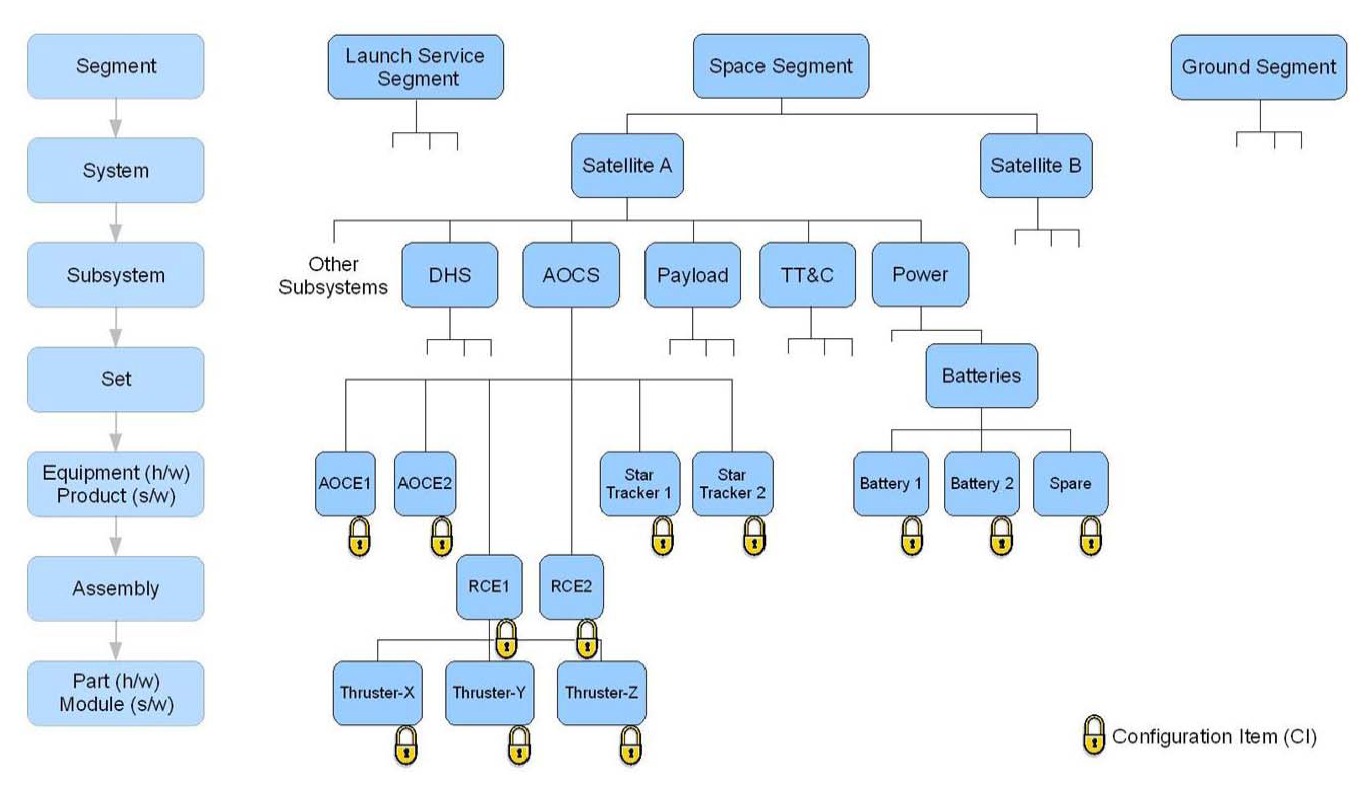
\includegraphics[scale=0.3]{fig/example_of_product_tree}
\caption{Example of Product Tree (ECSS)}
\label{fig:Example of Product Tree}
\end{figure}

\textbf{Work Breakdown Structure}: The work breakdown structure (WBS) is the most important structure to the project manager for managing the project in terms of cost, schedule, and technical content. The WBS divides the project into manageable smaller portions, which are expressed as work packages. The WBS has a hierarchical structure and the appropriate level of detail to which the project is broken down shall be defined by the project manager such that the WBS meets the needs of the project and the nature of the work; yet remains compact and not unnecessary complex. The WBS is derived from the product tree, but also takes into account supporting functions (such as the project management itself, testing activities, productions, etc.) that are necessary to carry out the project. An example of a WBS is provided in Figure \ref{fig:Example of Work Breakdown Structure}. Work related to manufacturing, assembly, integration and test of all product models shall be shown in the WBS.

\begin{figure}[h]
\centering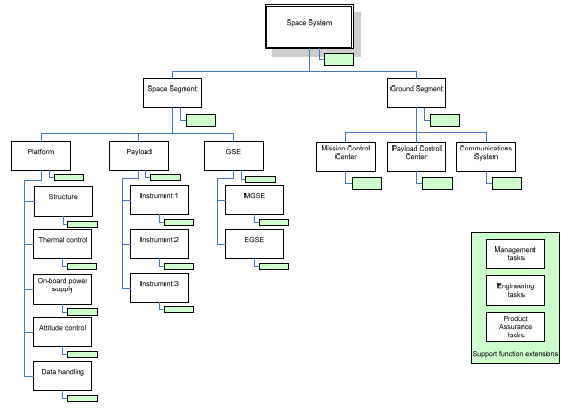
\includegraphics[scale=1.0]{fig/example_of_work_breakdown_structure}
\caption{Example of Work Breakdown Structure (ECSS)}
\label{fig:Example of Work Breakdown Structure}
\end{figure}

Each element in the WBS comprises a certain amount of work, requiring input and producing output. For each element in the WBS a work package description (WPD) shall be established (Section \ref{sec:Work Package Description}). A WP has to have clear definitions on its inputs, it required outputs, the tasks and approach of achieve the outputs, and other details. The purpose of a WPD on lower levels is particularly to separate the higher level complexity from it, such as to let the responsible person concentrate solely on the content of the WPD. A work package may be carried out by a team of people but only a single person is appointed as the responsible WPD manager.

\textbf{Organization Breakdown Structure}: The organization breakdown structure (OBS) depicts the project organization and also shows the contractual interfaces within the organization and to external parties. It shows the hierarchical structure of the key persons and all work package managers.

\subsubsection{Project Phases}

The life cycle of a space project is typically divided into distinct phases. Each phases contains activities to be carried out in the frame of this phase; however, some activities span over several phases. The phasing of a project follows the waterfall model: each phase follows its previous phase. The whole project in turn applies the "V model": From a top level description of the system, and subsequent derivation of requirements, down to its detailed definition; then going up again through verification of lower level then system level, and finally to its operation.

\begin{figure}[h]
\centering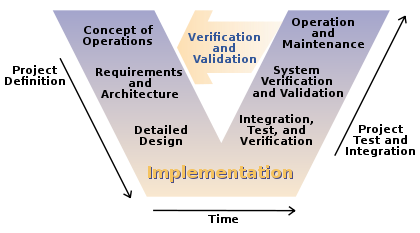
\includegraphics[scale=0.8]{fig/v_model}
\caption{V Model}
\label{fig:V Model}
\end{figure}

The distinct project phases are presented in the following sections. Reviews are held at the end of each phase (with some during a phase) to judge for the go-ahead to the next phase. See Figure \ref{fig:Project Phases and Reviews}.

\begin{figure}[h]
\centering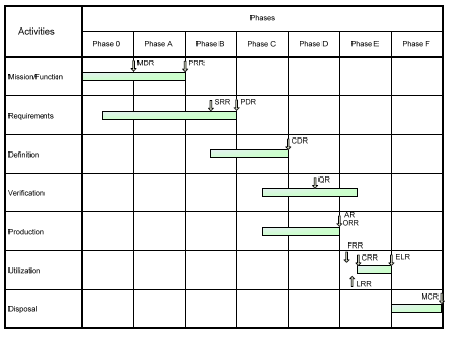
\includegraphics[scale=1.0]{fig/project_phases_and_reviews}
\caption{Project Phases and Reviews (ECSS)}
\label{fig:Project Phases and Reviews}
\end{figure}

\textbf{Phase 0: Mission Analysis and Needs Identification}: This phase is mainly carried out by the project initiator and the top level customer. The major tasks are:
\begin{itemize}
\item Elaborate the mission statement in terms of identification and characterization of the mission needs, expected performance, dependability and safety goals, and mission operating constraints with respect to the physical and operational environment.
\item Develop the preliminary requirements specification.
\item Identify possible mission concepts.
\item Perform preliminary assessment of programmatic aspects.
\item Perform preliminary risk assessment.
\end{itemize}

\textbf{Phase A - Feasibility}: This phase is carried out in order to provide the ground works for the feasibility of the project. The major tasks are:
\begin{itemize}
\item Establish the preliminary project management (PM), system engineering (SE), and product assurance (PA) plans.
\item Elaborate possible system and operations concepts.
\item Establish the function tree.
\item Assess the technical and programmatic feasibility of the possible concepts.
\item Identify critical technologies and propose pre-development activities.
\item Determine critical elements.
\item Propose the system and operations concept(s) and technical solutions, including model philosophy and verification approach, to be further elaborated during Phase B.
\item Elaborate risk assessment.
\end{itemize}

 It involves the establishment of the preliminary PM, SE, and PA plans, trade-off studies of different system concepts and architectures (including model philosophy and verification approach), the establishment of the function tree, the identification of critical technologies and pre-development activities, and the elaboration of the risk assessment.

\textbf{Phase B - Preliminary Definition}: The major tasks of this phase are:
\begin{itemize}
\item Finalize the PM, SE, and PA plans.
\item Elaborate the master schedule and baseline.
\item Elaborate the preliminary organizational breakdown structure.
\item Select the system and operations concept, as well as the technical solution, and the verification concept.
\item Establish the preliminary design definition for the selected concept.
\item Identify and define external interfaces.
\item Initiate pre-development work on critical technologies.
\item Initiate procurement of long lead items.
\item Finalize product tree, work breakdown structure, and specification tree.
\item Update risk assessment and conduct reliability and safety assessment.
\end{itemize}

\textbf{Phase C - Detailed Definition}: The activities of this phase are driven by the selected model philosophy and verification approach. The major tasks of this phase are:
\begin{itemize}
\item Completion of the detailed design definition of the system down to the lowest level.
\item Production, development testing and pre-qualification of selected critical elements.
\item Production and development testing of engineering models, as required
by the selected model philosophy and verification approach.
\item Completion of assembly, integration and test planning for the entire system.
\item Detailed definition of internal and external interfaces.
\item Issue of preliminary user manual.
\item Update of the risk assessment.
\end{itemize}

\textbf{Phase D - Qualification and Production}: The major tasks of this phase are:
\begin{itemize}
\item Complete manufacturing, assembly and testing of flight hardware/software and associated ground support hardware/software.
\item Complete verification program (qualification and acceptance stages).
\item Prepare system for delivery.
\end{itemize}

\textbf{Phase E - Operations and Utilization}: The activities of this phase depend widely on the type of project and mission. In general, the major tasks of this phase are:
\begin{itemize}
\item Perform all activities at space and ground segment level in order to prepare the launch.
\item Conduct all launch and early orbital operations.
\item Perform on orbit verification (including commissioning) activities.
\item Perform all on orbit operations in order to achieve the mission objectives and perform all ground segment and ground support activities in order to support the mission.
\item Finalize the disposal plan.
\end{itemize}

\textbf{Phase F - Disposal}: The major task of this phase is to implement the disposal plan.

\subsubsection{Reviews}

\begin{tabular}{l}
\textit{ECSS-M-ST-10-01 "Organization and conduct of reviews" \cite{ECSS-M-ST-10-01}} 
\end{tabular}

Reviews are milestones of a project to examine the status and completeness of the project at that point of time against the expected status. Normally, the review board includes external participants that further contribute with their objective view to the critical assessment of the project. Additionally, reviews can identify potential lessons learned.

Reviews are carried out throughout the project life cycle at all levels from mission to unit level. The review purpose, mandate and documentation vary for each particular project and for the specific phase or stage of activity of the project. 

\textbf{Review Bodies}: The participants of a review shall be composed of:
\begin{itemize}
\item The \textbf{review authority / review board}: Appointed by the customer, composed of members of customer organization and external participants that provide further objectiveness to the review.
\item The \textbf{review team}: Appointed by review authority, composed of people preferably with no direct involvement in the project. One single person of this team shall be appointed as review team leader.
\item The \textbf{project team}: Composed of all or a representative subset of the supplier team.
\end{itemize}

\textbf{Review Process}: The course of a review consists of the following steps:
\begin{enumerate}
\item The customer appoints the review authority, the review team, and review team leader.
\item The project team prepares the review procedure (Section \ref{sec:Review Procedure}), which is then subject to the customer's approval.
\item The project team supplies the review data packages subject to review to the review team. The project team is further responsible for the practical implementation of the review, including an optional kick-off meeting (for defining the review objectives), intermediate coordination meetings (as needed), and the final meeting involving all review bodies.
\item The review team reviews the documentation, identifies problems and makes recommendations or requests clarifications in the form of review item discrepancies (Section \ref{sec:Review Item Discrepancy}), and prepares a report (Section \ref{sec:Review Team Report}). 
\item After a certain period during which the project team can respond to the review team in order to close review item discrepancies (RIDs), the review authority will take the final disposition about open RIDs and issue its final report (Section \ref{sec:Review Authority Report}).
\end{enumerate}

\textbf{Mission Definition Review (MDR)}: The primary objective of this review is to release the mission statement and assess the preliminary technical requirements specification and programmatic aspects.

\textbf{Preliminary Requirements Review (PRR)}: The primary objectives of this review are:
\begin{itemize}
\item Release of preliminary management, engineering and product assurance plans.
\item Release of the technical requirements specification.
\item Confirmation of the technical and programmatic feasibility of the system concept(s).
\item Selection of system and operations concept(s) and technical solutions, including model philosophy and verification approach, to be carried forward into Phase B.
\end{itemize}

\textbf{System Requirements Review (SRR)}: This review is held during the course of Phase B. The primary objectives of this review are:
\begin{itemize}
\item Release of updated technical requirements specifications.
\item Assessment of the preliminary design definition.
\item Assessment of the preliminary verification program.
\end{itemize}

\textbf{Preliminary Design Review (PDR)}: The primary objectives of this review are:
\begin{itemize}
\item Verification of the preliminary design of the selected concept and technical solutions against project and system requirements.
\item Release of final management, engineering and product assurance plans.
\item Release of product tree, work breakdown structure and specification tree.
\item Release of the verification plan (including model philosophy).
\end{itemize}

\textbf{Critical Design Review (CDR)}: The primary objectives of this review are:
\begin{itemize}
\item Confirm compatibility with external interfaces.
\item Release the final design.
\item Release assembly, integration and test planning.
\item Release flight hardware/software manufacturing, assembly and testing.
\item Release of user manual.
\end{itemize}

\textbf{Qualification Review (QR)}: The primary objectives of this review are:
\begin{itemize}
\item Confirm that the verification process has demonstrated that the design, including margins, meets the applicable requirements.
\item Verify that the verification record is complete at all levels of the system.
\item Verify the acceptability of all waivers and deviations. 
\end{itemize}

\textbf{Acceptance Review (AR)}: The primary objectives of this review are:
\begin{itemize}
\item Confirm that the verification process has demonstrated that the product is free of workmanship errors and is ready for subsequent operational use.
\item Verify that the acceptance verification record is complete at all levels of the system.
\item Verify that all deliverable products are available per the approved deliverable items list.
\item Verify the "as-built" product and its constituent components against the required "as designed" product and its constituent components.
\item Verify the acceptability of all waivers and deviations.
\item Verify that the Acceptance Data Package is complete.
\item Authorize delivery of the product.
\item Release the certificate of acceptance.
\end{itemize}

\textbf{Operational Readiness Review (ORR)}: The primary objectives of this review are:
\begin{itemize}
\item Verify readiness of the operational procedures and their compatibility with the flight system.
\item Verify readiness of the operations teams.
\item Accept and release the ground segment for operations.
\end{itemize}

\textbf{Flight Readiness Review (FRR)}: The flight readiness review is conducted prior to launch. The objective of this review is to verify that the flight and ground segments including all supporting systems such as tracking systems, communication systems and safety systems are ready for launch.

\textbf{Launch Readiness Review (LRR)}: The launch readiness review is conducted just prior to launch. The objective of this review is to declare readiness for launch of the launch vehicle, the space and ground segments including all supporting systems such as tracking systems, communication systems and safety systems and to provide the authorization to proceed for launch.

\textbf{Commissioning Result Review (CRR)}: The commissioning result review is held at the end of the commissioning as part of the in-orbit stage verification. It allows declaring readiness for routine operations/utilization. This Review is conducted following completion of a series of on-orbit tests designed to verify that all elements of the system are performing within the specified performance parameters. Successful completion of this review is typically used to mark the formal handover of the system to the project initiator or to the system operator.

\textbf{End of Life Review (ELR)}: This review is conducted to verify that the mission has completed its useful operation or service and to ensure that all on-orbit elements are configured to allow safe disposal.

\textbf{Mission Close-Out Review (MCR)}: This review is conducted to ensure that all mission disposal activities are adequately completed.

\subsection{Configuration Management}
\label{sec:Configuration Management}

\begin{tabular}{l}
\textit{ECSS-M-ST-40 "Configuration and information management" \cite{ECSS-M-ST-40}}
\end{tabular}

Configuration management (CM) is the process for establishing and maintaining a consistent record of a system's functional and physical characteristics ("as built") compared to its design and operational requirements ("as designed"). Configuration management is applied throughout the entire life cycle of the product and allows to know at any time the technical description of a product using approved documentation. It helps to record, control, and provide traceability of the evolution in the technical description of a system and ensures the consistency of internal interfaces. It further allows to verify and demonstrate to all actors that documentation is and remains the exact image of the products it describes.

Configuration management interfaces with engineering, product assurance, manufacturing and production, and operations. The supplier produces the \textbf{configuration management plan} (Section \ref{sec:Configuration Management Plan}). The four main tasks of CM are described in the following sections.

\subsubsection{Configuration Identification}

The product tree is used for the selection of \textbf{configuration items} (CIs). CIs fall in two categories: developed or non-developed. The latter is for products that are off-the-shelf, or available from previous projects. Configuration items are identified at various levels of the product tree. There are no fixed rules for which item to select as configuration item, but each selected CI is subject to full configuration management. One generally selects those items that are likely subject to configuration change, be it in hardware or software configuration, or items that the configuration management wishes to have control over (such as the baseline of the ground infrastructure). Each CI shall be labelled with a unique identifier, composed of a part identifier and a serial or lot number (for hardware) or version number (for software). The identifier shall be placed on the item itself if possible, or linked to it. The list of all selected configuration items is maintained in the \textbf{configuration item list} (Section \ref{sec:Configuration Item List}).

\subsubsection{Configuration Control}

During the life cycle of the project several configuration baselines are defined and agreed upon. Configuration control is the process for controlling the evolution of those baselines.

Changes to configuration items can only be done through change control procedures. Changes on \textbf{requirements} are done through \textbf{change requests} or \textbf{change proposals}. Change requests (Section \ref{sec:Change Request}) come from the customer (e.g. for evolution of requirements), whereby change proposals (Section \ref{sec:Change Proposal}) come from the supplier (e.g. self initiated improvement of design). The \textbf{configuration control board}, which can be a single person or a team appointed by the project manager, takes decision on those requests; and in case of major departures from the baseline it does this in coordination with the customer.

Before production, the supplier may request changes to the \textbf{configuration items} through \textbf{requests for deviation}. A request for deviation (Section \ref{sec:Request for Deviation}) is used to agree on the planned departure from the customers requirement that is part of an approved configuration baseline. After production, when the supplier discovers non-conformance of configuration items, a \textbf{requests for waiver} may be applied.  A request for waiver (Section \ref{sec:Request for Waiver}) is used to agree on the use and/or delivery of a product that is not conform to the approved product configuration baseline.

For changes during the operational phase of the mission the same principle apply.

\subsubsection{Configuration Status Accounting}

Configuration status accounting provides the ability to record and report on the configuration baselines at any moment of time. An important tool for this is the \textbf{configuration item data list} (Section \ref{sec:Configuration Item Data List}) that lists all relevant technical documents and their version number for each configuration item (including references to lower level configuration items). The \textbf{as-built configuration data list} (Section \ref{sec:As-Built Configuration Data List}) is a document to act as reporting instrument defining the physical as-built status of each configuration item and listing any discrepancies to the configuration item data list (CIDL). The \textbf{software configuration file} (Section \ref{sec:Software Configuration File}) is used for reviews, and created for each configuration item that involves software development.

\subsubsection{Configuration Verification}

The project reviews (and possibly occasional audits) are used for verification of the configuration.

\subsection{Information Management}

\begin{tabular}{l}
\textit{ECSS-M-ST-40 "Configuration and information management" \cite{ECSS-M-ST-40}}
\end{tabular}

Information management is concerned with the life cycle of documents, that is the creation, collection, review, delivery, storage, archiving, and retrieval of them. All documents are managed electronically.

\subsubsection{Document Reference Number}

Each newly created document is assigned a unique reference number. The structure of such reference number is mission specific and may, for example, be structured as

\texttt{<ORG>-<Project>-<WBS\#>-<Type>-<Number>}. 

For the first "minutes of meeting" document regarding the element "5500" in the work breakdown structure of  project "CSAT" from organization "CORG" this yields the reference number 

\texttt{CORG-CSAT-5500-MIN-0001}. 

A list of ISO conform identifiers for element "Type" is given in Section \ref{sec:Common Document Types}.

\subsubsection{Document Status}

When a new document is created and assigned a reference number, it bears the status "in preparation". It is considered preliminary and cannot be used for binding agreements. When it is complete, it will be submitted for review and bears the status "under review". As the outcome of the review the documents status may change to "rejected" (if it did not pass the review), "superseded" (if it was replaced by another document), or "approved". The document is then digitally signed.

\subsubsection{Document Version}

Once approved the document is valid for use and for binding agreements. Any modification to the document implies a new version. The version of a document is updated in the document  and the document file is appended by its issue number and revision number in the form \_iXrY, where X is the issue and Y is the revision. Before the approval of a document its issue number is zero (0) and the revision number shall start with a one (1) and be incremented upwards. The first approved issue of a document is \_i1r0. Minor changes affect the revision whereas major changes (such as design reviews) change the issue. For the above example, the second issue and first revision of the document would yield the complete reference as 

\texttt{CORG-CSAT-5500-MIN-0001\_i2r1}.

Every change of a document shall be approved and digitally signed to take affect.

\subsubsection{File Formats}

File formats for electronic documents are preferably open formats. Some examples are:

\begin{itemize}
\item PDF for signed read only documents
\item OpenDocument formats for editable text documents, spreadsheets, presentations
\item JPEG for photographic images
\item PNG or TIFF for technical images
\item SVG for vector graphics
\item ZIP for packed archives
\end{itemize}

For other types of data (such as CAD drawings, PCB layout, circuit schematics) open exchange formats are preferred where available.

\subsubsection{File Exchange}

File exchange is preferably done using ZIP files as container.

\subsubsection{Document Management System}

The document management system shall ensure that project information/documentation is

\begin{itemize}
\item preserved from damage or loss,
\item accessible and retrievable,
\item access controlled to authorized users.
\end{itemize}

\subsection{Cost Management}

\begin{tabular}{l}
\textit{ECSS-M-ST-60 "Cost and schedule management" \cite{ECSS-M-ST-60} }
\end{tabular}

Cost management includes the activities to complete the project with a defined budget, namely through cost estimation and planning, cost control, and cost reporting. It facilitates the predication of potential budget deviations and the implementation of countermeasures to avoid cost overruns. Cost management is strongly tied to schedule management. Cost management may establish a business agreement structure diagram to identify the cost reporting relationships between respective customers and suppliers. A useful tool for supporting cost management is the cost breakdown structure (Annex A of ECSS-M-ST-60 provides details).

\subsubsection{Cost Estimating and Planning}

Cost estimating is the process of determining the expected costs of a project. Different methods for cost estimation can be applied. Commonly, a top-down approach (i.e. referring to cost data from similar projects) is used at early phases of the project and bottom-up approaches (i.e. analyzing each individual work package and summing it all up) at later phases. In particular for the bottom-up approach, the work breakdown structure of the project is an important input. This transforms the work breakdown structure into a cost breakdown structure. Cost estimations (see Annex E of ECSS-M-ST-60) are supplied to the customer at agreed milestones and to be updated throughout the project.

\subsubsection{Cost Control}

The customer approved cost estimation forms the \textbf{original baseline cost plan}, which is updated continuously as the \textbf{current baseline cost plan}. In order to allow better control over the costs, two key numbers are continuously updated: the estimate at completion (EAC) and the estimate to completion (ETC). The EAC gives an estimate of the total expenses of the project upon its completion, whereas the ETC is the total expenses for work to be performed from now until the work is completed.

\subsubsection{Cost Reporting}

Depending on the agreement, the supplier periodically submits reports about the cost evolution to the customer. These are namely the original and current baseline cost plan, and the EAC and ETC numbers.

\subsection{Schedule Management}

\begin{tabular}{l}
\textit{ECSS-M-ST-60 "Cost and schedule management" \cite{ECSS-M-ST-60}}
\end{tabular}

Schedule management includes the activities to complete a project within a defined time, namely through establishment of the schedule, schedule control, and schedule reporting. 

\subsubsection{Schedule Definition}

Scheduling takes into account the work to be performed versus the available resources to implement this work and produces a schedule down to sufficient detail. A schedule is actually a network of activities and milestones, together with the relationships between them (see Annex B of ECSS-M-ST-60 for details). For instance, some activities may run in parallel but some activities may depend on the completion of other activities before they can start. 

The work breakdown structure is the input to the schedule definition. The activities are put in sequence and linked to each other reflecting the logical dependencies between them. Next, the duration is estimated for each activity and the required resources. This is then translated into a schedule using a working calendar as basis, that specifies the working hours, holidays, and so on. 

There are also a number of milestones to be placed in the schedule. Traditionally they serve as "gates", which need to be passed in order to proceed with following activities. At minimum, the following milestones are defined: start/end of project, reviews, delivery dates, and business agreement milestones. Figure \ref{fig:Example of Gantt Chart} shows an example Gantt chart as outcome of the schedule definition process.

\begin{figure}[h]
\centering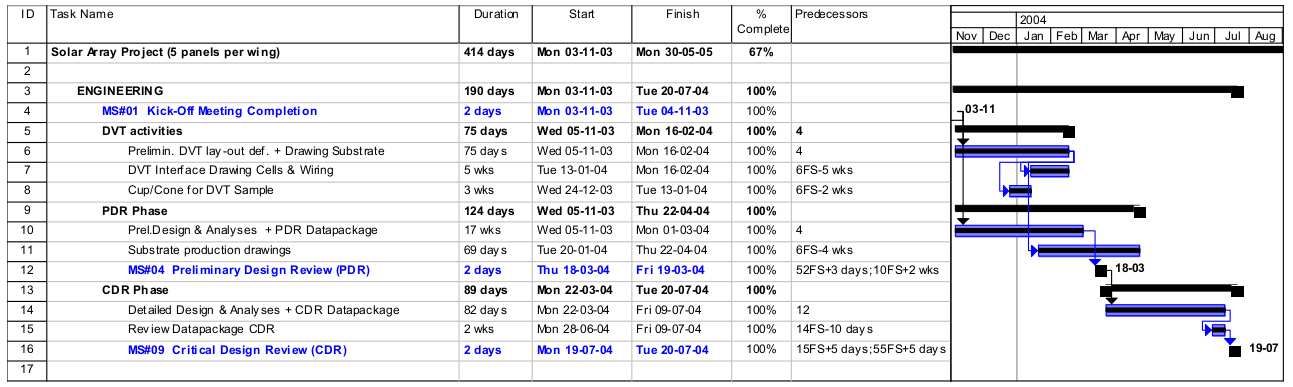
\includegraphics[scale=0.3]{fig/example_of_gantt_chart}
\caption{Example of Gantt Chart (ECSS)}
\label{fig:Example of Gantt Chart}
\end{figure}

\subsection{Schedule Control}

Two schedules are used for schedule control: the baseline schedule and the current working schedule. 

The \textbf{baseline schedule} is the reference schedule that was approved by the customer and allows for timely completion of the project or project phase. It is established through the schedule definition task as already explained. It contains as a minimum the milestones, description and duration of activities, the start and finish dates of activities, and the identification of the critical path. The critical path is the sequence of project network activities which add up to the longest overall duration. This determines the shortest time possible to complete the project.

The \textbf{current working schedule} on the other hand documents the actual status of completed and planned activities, and is updated continuously. It reflects the most realistic view of the project status.

Both schedules are identical at start of the project. As the project progresses, the current working schedule can differ, due to differences in planned and actual progress. This identification of those differences form the basis for progress assessment and the possible implementation of countermeasures to bring the schedule back on track.

\subsubsection{Schedule Reporting}

Schedule reporting is needed to inform the customer about the project progress. The regularity of such reporting is agreed between supplier and customer, and comprise at a minimum details on: activities started/completed, completion forecast for ongoing activities, and an assessment of the logical between activity relationships (see Annex C of ECSS-M-ST-60 for details).

Such progress updates may be conveyed during progress meetings, progress reports, and reviews. Independent from such regular progress updates, if there are major delays in the schedule then the customer shall be informed immediately.

\subsection{Integrated Logistic Support}

\begin{tabular}{l}
\textit{ECSS-M-70 "Integrated logistic support" \cite{ECSS-M-70}}
\end{tabular}

Integrated logistic support (ILS) is a process for developing material resources and services essential to support development, operation and maintenance. The purpose of it is to maintain the technical and availability performance levels while respecting safety constraints and optimizing overall life cycle cost.

Factors of logistic needs are usually: support facilities and equipment, support tools (including software), personnel skills and training, and maintenance plans.  

Integral part of ILS is also inventory control, namely for EEE parts, consumables, equipment, and custom items.

\subsection{Risk Management}
\label{sec:Risk Management}

\begin{tabular}{l}
\textit{ECSS-M-ST-80 "Risk management" \cite{ECSS-M-ST-80}}
\end{tabular}

Risks impact the cost, schedule, or technical performance of a project and therefore present a danger to project success. The objective of risk management is to identify, assess, reduce, accept, and control risks. Proper risk management allows optimization of the overall cost of a project.

The mitigation of risks already starts with the implementation of a systematic methodology for all space project disciplines, namely project management, product assurance, system engineering, and mission operations. Risk management is to be carried out on a day-to-day basis.

The risk management process includes the establishment of a risk management policy, the identification and assessment of risks, the decision on risks, and risk monitoring. The later three steps are carried out in a continuous loop throughout the project life cycle.

Policy
$\rightarrow$ Identify
$\rightarrow$ Decide
$\rightarrow$ Monitor
$\rightarrow$ Identify
$\rightarrow$ etc.

\subsubsection{Risk Management Policy and Plan}

The \textbf{risk management policy document} (Section \ref{sec:Risk Management Policy Document}) describes the objective and principles of risk management in the context of the project. It specifies on a high level the criteria for classification and acceptance of risks. This includes for example the definition of scoring schemes for risk likelihood and severity, and the risk indexing.

The \textbf{risk management plan} (Section \ref{sec:Risk Management Plan}) on the other hand specifies how risk management is implemented, such as roles and responsibilities of people.

\subsubsection{Risk Identification and Assessment}

Risk identification is to be performed in all disciplines and levels of the project. Risks may be of technical, cost, schedule, or other nature. Each member of the engineering team shall be responsible for continuously assessing the risks on their part of the project through the project life cycle, recording this in the form of a project-level risk register, and communicating the risk assessment to the project manager and system engineer.

Every identified risk scenario should be assessed in terms of its causes and consequences, in accordance with the risk policy. In particular, the risk shall be further quantified in terms of severity, likelihood, and so on, and added to the \textbf{risk assessment report} (Section \ref{sec:Risk Assessment Report}).

\subsubsection{Decision on Risks}
 
Identified risks may be either mitigated or accepted. Usually, risks that have minor impact but are costly to avoid are accepted. Risks however which do have a more severe impact on the project and are unacceptable should be avoided by all means possible. If avoidance is not feasible, then this must be communicated to the customer.

The project manager shall maintain the \textbf{risk register} (Section \ref{sec:Risk Register}) and delegate to the system engineer the responsibility to properly address these risks with the engineering team through the planning of specific activities to mitigate them. The project manager and system engineer shall then assign the responsibility for carrying out the risk mitigation actions to individual members of the project engineering team.
 
\subsubsection{Risk Monitoring}

The project manager shall use the risk register to regularly communicate the project risks and mitigation action plans. Periodically all identified risks shall be re-assessed. Further, the implementation of risk reduction performance shall be reviewed over time. One way to visualize this is the use of a risk trend chart. 
  
\clearpage
\section{Deliverables}
\label{sec:Project Management Deliverables}

\subsection{Documents per Review}
\begin{table}[h]
\centering
\begin{tabular}{l c c c c c c c c c}
\toprule
\textbf{Phase} & \textbf{0} & \textbf{A} & \multicolumn{2}{c}{\textbf{B}} & \textbf{C} & \multicolumn{2}{c}{\textbf{D}} & \multicolumn{2}{c}{\textbf{E}} \\
\textbf{Review} & \textbf{MDR} & \textbf{PRR} & \textbf{SRR} & \textbf{PDR} & \textbf{CDR} & \textbf{QR} & \textbf{AR} & \textbf{ORR} & \textbf{FRR} \\
\midrule
Project management plan         &   & •  & • & • &   &   &   &   &   \\
\hline
Product tree					&   & • & • & • & • & • & • &   &   \\
\hline
Work breakdown structure 		&   & • & • & • &   &   &   &   &   \\
\hline
Work package description     	&   & • & • & • &   &   &   &   &   \\
\hline
Schedule						& • & • & • & • & • & • & • & • & • \\
\hline
Cost estimate report			&   & • & • & • &   &   &   &   &   \\
\hline
Config. management plan 		&   & • & • & • &   &   &   &   &   \\
\hline
Config. item list				&   &   &   & • & • &   &   &   &   \\
\hline
Config. item data list			&   &   &   & • & • & • & • &   &   \\
\hline
As-built config. list			&   &   &   &   &   & • & • &   &   \\
\hline
Software config. list			&   &   &   & • & • & • & • &   &   \\
\hline
Config. status acc. reports		&   &   &   & • & • & • & • &   &   \\
\hline
Risk management policy doc.	    & • & • & • & • &   &   &   &   &   \\
\hline
Risk management plan			& • & • & • & • &   &   &   &   &   \\
\hline
Risk assessment report			&   & • & • & • & • & • & • & • & • \\
\bottomrule
\end{tabular}
\caption{Management Documents required per Review}
\end{table}

\subsection{Documents per Request}
\begin{itemize}
\item Cost breakdown structure
\item Schedule progress report
\item Cost estimating plan
\item Inventory record
\item Cost and manpower report
\item Risk register
\end{itemize}